% =====================================================================
%  Williamson 5 (flow over a mountain) — long-time structure preservation.
%  Deterministic, BDM2/DG1, cPG(P1), ref 5, dt = 135 s, t = 15 days.
%  Diagnostics from w5_diagnostics_pure.csv. Requires \usepackage{graphicx}.
% =====================================================================

\begin{figure}[htbp]
  \centering
  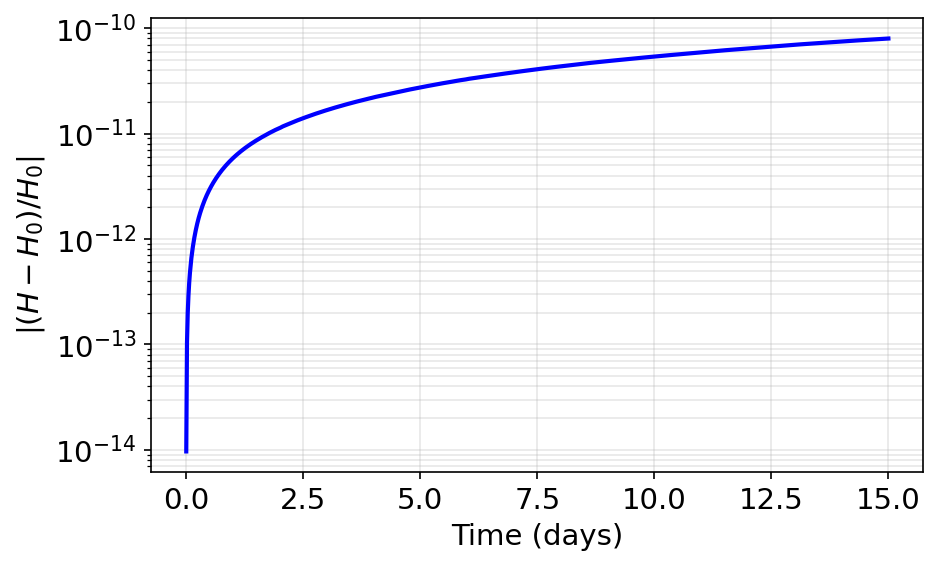
\includegraphics[width=0.8\textwidth]{w5_energy_longtime.png}
  \caption{Long-time energy conservation for the Williamson test case~5 (flow over
    an isolated mountain), deterministic, BDM$_2$/DG$_1$, cPG($P_1$) on refinement
    level~5 with $\Delta t = 135$\,s, integrated to $t = 15$ days. The relative
    energy drift $|(H-H_0)/H_0|$ remains at the solver/round-off level
    ($\le 8\times10^{-11}$) throughout, with no secular growth, even though the
    mountain continuously generates gravity waves and a lee vortex train. This is
    the strongest form of the energy-conservation claim: the fully discrete
    space--time scheme conserves energy over a long integration of a persistently
    active flow.}
  \label{fig:w5-energy-longtime}
\end{figure}

\begin{figure}[htbp]
  \centering
  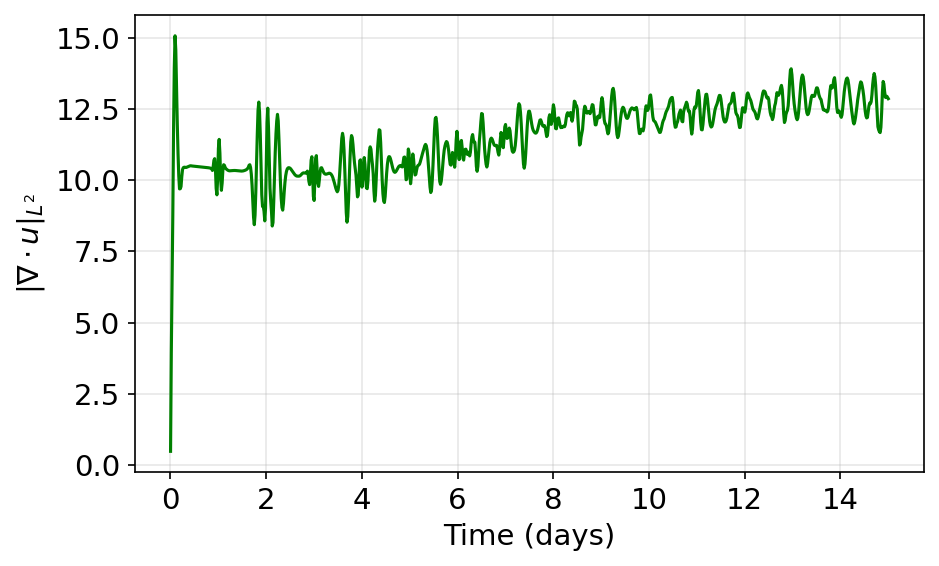
\includegraphics[width=0.8\textwidth]{w5_div_longtime.png}
  \caption{Velocity divergence $\|\nabla\cdot u\|_{L^2}$ versus time for the
    Williamson test case~5 run of Fig.~\ref{fig:w5-energy-longtime}. After the
    initial gravity-wave adjustment to the mountain forcing the divergence settles
    into a bounded oscillation (range $\approx 0.5$--$15$) tracking the wave
    activity, with no secular growth over the 15-day integration.}
  \label{fig:w5-div-longtime}
\end{figure}

\begin{figure}[htbp]
  \centering
  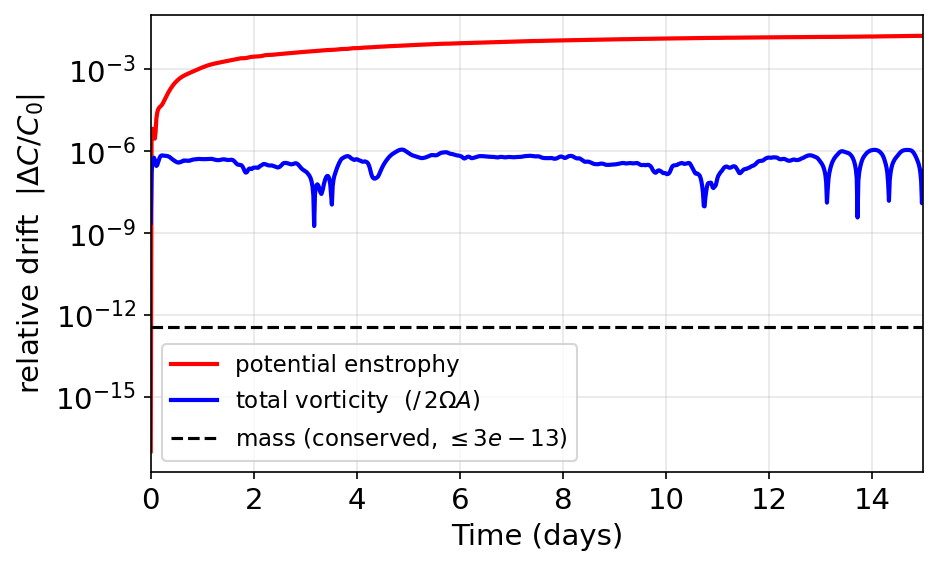
\includegraphics[width=0.8\textwidth]{w5_casimirs.png}
  \caption{Conservation of the Casimir invariants for the Williamson test case~5 run
    of Fig.~\ref{fig:w5-energy-longtime}: relative drift of total mass
    $M=\int D$, potential enstrophy $Z=\int q^2 D/2$ with $q=(\nabla^\perp\!\cdot
    u+f)/D$, and total absolute vorticity $\int(\nabla^\perp\!\cdot u+f)$ (the last
    normalised by the planetary scale $2\Omega A$, $A$ the sphere area, since its
    conserved value is zero). \textbf{Mass is conserved to round-off}
    ($\sim\!3\times10^{-13}$) and \textbf{total vorticity stays bounded at
    $\sim\!10^{-6}$} of the planetary scale, both consistent with exact
    preservation by the compatible finite-element spaces. \textbf{Potential
    enstrophy is not exactly conserved} by an energy-conserving scheme and exhibits
    a slow, bounded drift ($+1.7\%$ over 15 days) -- the expected behaviour, shown
    here without adjustment.}
  \label{fig:w5-casimirs}
\end{figure}

\begin{figure}[htbp]
  \centering
  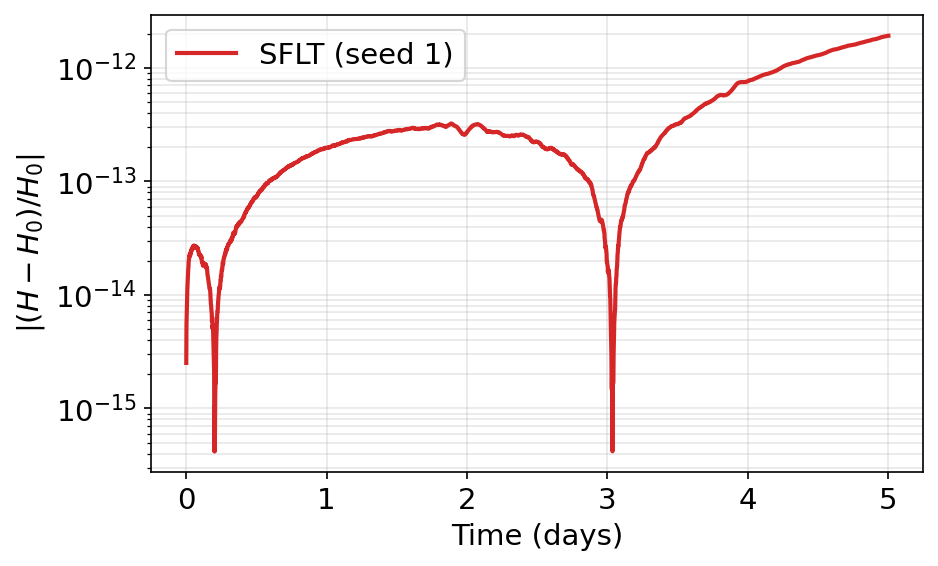
\includegraphics[width=0.8\textwidth]{w5_sflt_energy.png}
  \caption{Energy conservation under SFLT stochastic forcing for the Williamson test
    case~5, BDM$_2$/DG$_1$, cPG($P_1$) on refinement level~5 with $\Delta t = 135$\,s,
    integrated to $t = 5$ days (single realisation, seed~1). Despite the continuous
    injection of divergence-free noise into the momentum equation, the relative
    energy drift $|(H-H_0)/H_0|$ remains at the solver/round-off level
    ($\le 2\times10^{-12}$) throughout, matching the deterministic behaviour of
    Fig.~\ref{fig:w5-energy-longtime}. This confirms that the discrete
    energy-conservation property of the scheme carries over to the stochastic
    setting, as expected from the energy-preserving structure of SFLT.}
  \label{fig:w5-sflt-energy}
\end{figure}

\begin{figure}[htbp]
  \centering
  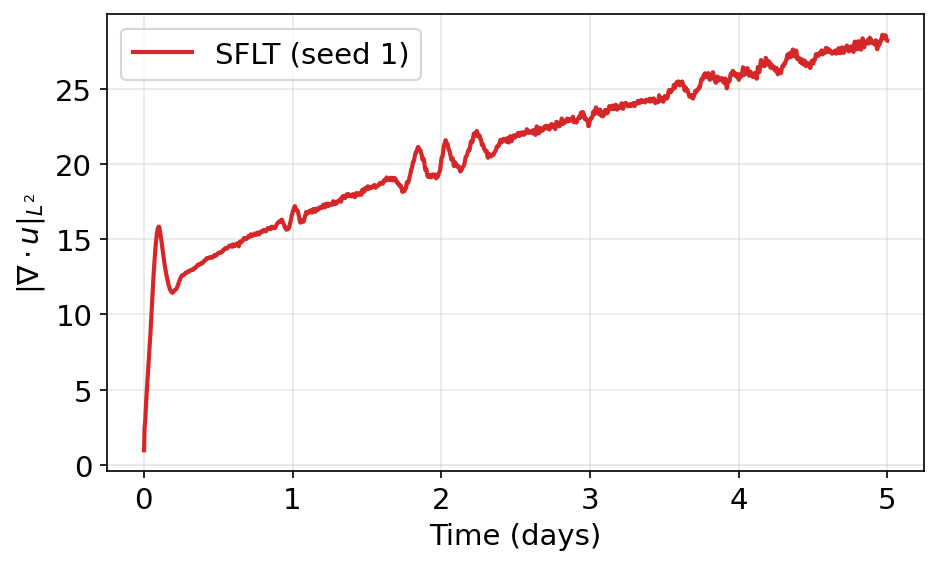
\includegraphics[width=0.8\textwidth]{w5_sflt_div.png}
  \caption{Velocity divergence $\|\nabla\cdot u\|_{L^2}$ under SFLT forcing for the
    Williamson test case~5 run of Fig.~\ref{fig:w5-sflt-energy}. The stochastic
    forcing excites the compressible modes of the resolved flow: the divergence
    grows from the mountain-driven baseline (cf.\ Fig.~\ref{fig:w5-div-longtime})
    to $\approx 28$ over 5 days, with the noise superposed on the deterministic
    gravity-wave activity. The scheme remains stable throughout without any
    filtering or dissipation.}
  \label{fig:w5-sflt-div}
\end{figure}
